\documentclass[12pt,a4paper]{article}

\usepackage[czech]{babel}
\usepackage[utf8]{inputenc}
\usepackage{float}
\usepackage{graphicx}
\usepackage[left=3cm,right=2cm, top=3cm,bottom=2cm]{geometry}
\usepackage{textcomp}
\usepackage[fleqn]{amsmath}
\usepackage{caption}
\linespread{1.3}
\usepackage{hyperref}
\usepackage{xcolor}
\definecolor{linkcolor}{HTML}{799B03}
\definecolor{urlcolor}{HTML}{799B03}
\hypersetup{pdfstartview=FitH,  linkcolor=linkcolor,urlcolor=urlcolor, colorlinks=true}

% neodsazovat nové odstavce
\setlength{\parindent}{0pt}

\begin{document}

	%%%%%%%%%%%%%%%%%%%%%%%%%%%%%%%%%%%%%%%%%%%%%%%% Titulní list %%%%%%%%%%%%%%%%%%%%%%%%%%%%%%%%%%%%%%%%%%%%%%%%

	\begin{titlepage}
		\begin{center}
			\textsc{\LARGE Vysoké Učení Technické v Brně} \\[0.5cm]
			{\LARGE Fakulta informačních technologií}
			\vspace{2cm}
			\begin{figure}[H]
				\center
\includegraphics[width=0.8\linewidth]{pictures/VUT} 
			\end{figure}

			\vspace{1cm}

			\textsc{\LARGE Praktické aspekty vývoje software} \\[0.5cm]
			\textsc{\LARGE 2017/2018} \\[3.5cm]

			\textbf{{\LARGE Projekt - kalkulačka}}
		\end{center}
		\vfill
		\begin{flushleft} 
			\large
			Bali Filip (xbalif00) \\
			Holkova Natalia (xholko02) \\
			Novak Matej (xnovak2f) \\
			Shamardin Egor (xshama00)
			\hfill
			Brno, \today
		\end{flushleft}
	\end{titlepage}

	%%%%%%%%%%%%%%%%%%%%%%%%%%%%%%%%%%%%%%%%%%%%%%%% Obsah %%%%%%%%%%%%%%%%%%%%%%%%%%%%%%%%%%%%%%%%%%%%%%%%

	\section*{\LARGE Obsah}
	\begin{flushleft}
		\textbf{1) Úvod .....................................................................................................2} \\
		\vspace{5mm}
		\textbf{2) Instalace, odinstalace programu .........................................................3-7} \\
		\vspace{5mm}
		\textbf{3) Jak pracovat s programem.....................................................................8} \\
		\vspace{5mm}
		\textbf{4) Závěr......................................................................................................9} \\
	\end{flushleft}

	
	\newpage
%%%%%%%%%%%%%%%%%%%%%%%%%%%%%%%%%%%%%%%%%%%%%%%% Úvod %%%%%%%%%%%%%%%%%%%%%%%%%%%%%%%%%%%%%%%%%%%%%%%%	
	\section*{\LARGE Úvod}
	
	\hspace{1cm}
	\textbf{Tento dokument slouží jako příručka pro uživatele, které rozhodli použit kalkulačku od týmů Baseballka. Dokument popisuje jednoduchý postup pro instalaci kalkulačky, obrázky pro představu.}\\
	 \hspace{1cm} 
	 \textbf{S pomoci kalkulačky můžeme provádět různé operace:} \\
	 1) Násobení, dělení, odčítání, sečtení \\
	 2) Výpočet druhé odmocniny		\\
	 3)	Umocňování	\\
	 4)	Logaritmus o základu 10 \\
	 5) Faktorial	
	
	\begin{figure}[H] 
		\center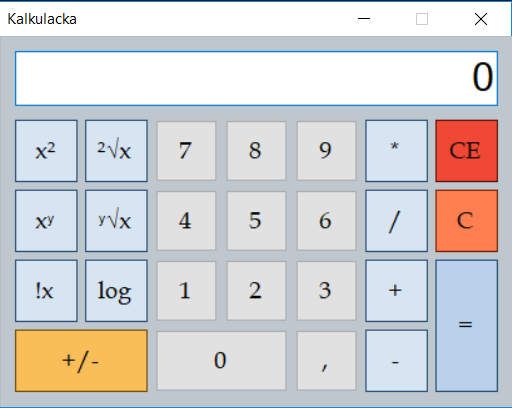
\includegraphics[width=0.6\linewidth]{pictures/look}
		\caption{Tak vypadá kalkulačka} 
	\end{figure}
	
	\newpage
	
%%%%%%%%%%%%%%%%%%%%%%%%%%%%%%%%% Instalace, odinstalace programu %%%%%%%%%%%%%%%%%%%%%%%%%%%%%%%%%%%%%	
	\section*{\LARGE Instalace, odinstalace programů}
	
	
	\textbf{Kroky pro instalaci:}
	\begin{enumerate}
	\item Stáhnete soubor install
	\item Po otevíraní adresaře install otevřite adresař "Release"
	\begin{figure}[H]
		\center
\includegraphics[width=0.8\linewidth]{pictures/2} 
	\end{figure}
	\item Po otevření "Release", spusite "setup.exe"
	\begin{figure}[H]
		\center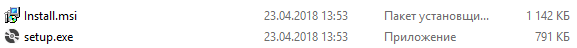
\includegraphics[width=0.8\linewidth]{pictures/3} 
	\end{figure}
	\item Začíná instalace
	\begin{figure}[H]
		\center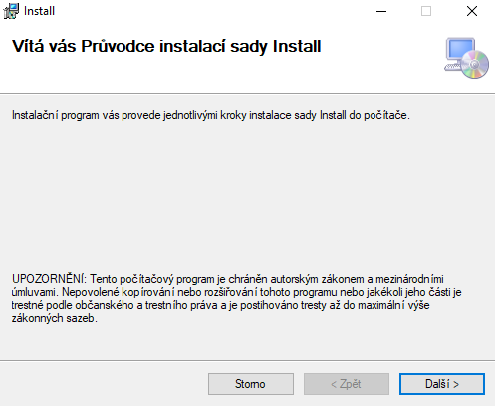
\includegraphics[width=0.8\linewidth]{pictures/4}
		\caption{Na uvodní obrazovce kliknite na tlačitko "Další"} 
	\end{figure}
	\begin{figure}[H]
		\center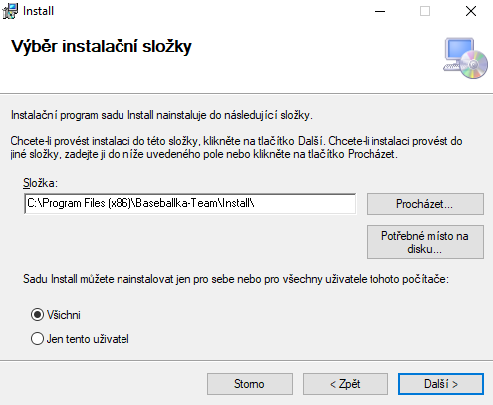
\includegraphics[width=0.8\linewidth]{pictures/5}
		\caption{Mužete vybrat cestu, pak klikneme na "Další"}
	\end{figure}
	\begin{figure}[H]
		\center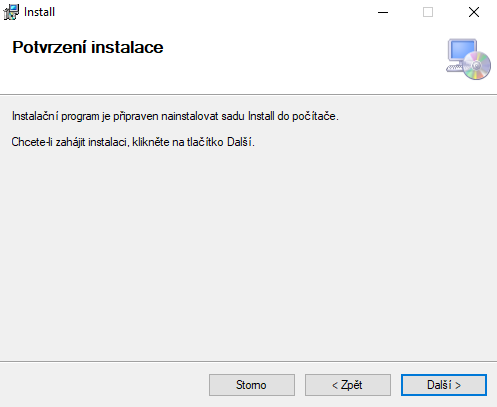
\includegraphics[width=0.8\linewidth]{pictures/6}
		\caption{Pro potvrzení instalace klikneme na "Další"}
	\end{figure}
	\begin{figure}[H]
		\center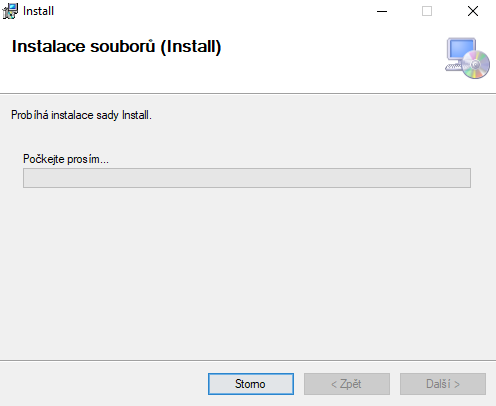
\includegraphics[width=0.8\linewidth]{pictures/7}
		\caption{Začíná instalace. Může trvat několik minut}
	\end{figure}
	\begin{figure}[H]
		\center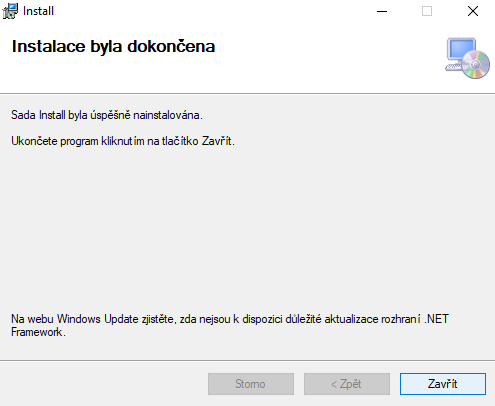
\includegraphics[width=0.8\linewidth]{pictures/8}
		\caption{Po okončení kliknete na "Zavřit"}
	\end{figure}
	\begin{figure}[H]
		\center
\includegraphics[width=0.1\linewidth]{pictures/9}
		\caption{Teď na ploše objeví štítek, po kliknutí ktereho otevří kalkulačka}
	\end{figure}
	\item Program byl nainstalovan
	\end{enumerate}
	
	\textbf{Odinstalace:}
	\begin{enumerate}
	\item Pro odinstalace stisknete "setup.exe"
	\begin{figure}[H]
		\center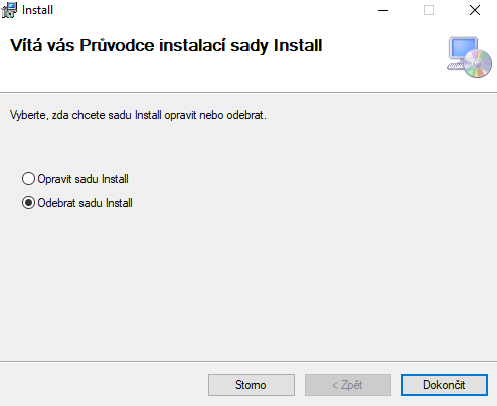
\includegraphics[width=0.8\linewidth]{pictures/10}
		\caption{Pro odinstalaci vyberte "Odebrat sadu install" a kliknete "Dokončit"}
	\end{figure}
		\begin{figure}[H]
		\center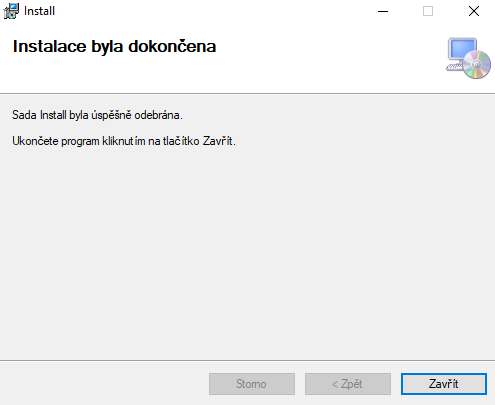
\includegraphics[width=0.8\linewidth]{pictures/11}
		\caption{Po dokončení kliknete "Dokončit"}
	\end{figure}
	\item program byl odinstalovan
	\end{enumerate}
	\newpage
%%%%%%%%%%%%%%%%%%%%%%%%%%%%%%%%%%%%% Jak pracovat s programem %%%%%%%%%%%%%%%%%%%%%%%%%%%%%%%%%%%%%%%%	
	\section*{\LARGE Jak pracovat s programem}
	
	\textbf{Pri spouštení programů otevíra kalkulačka(obr.10).}
	\begin{figure}[H] 
		\center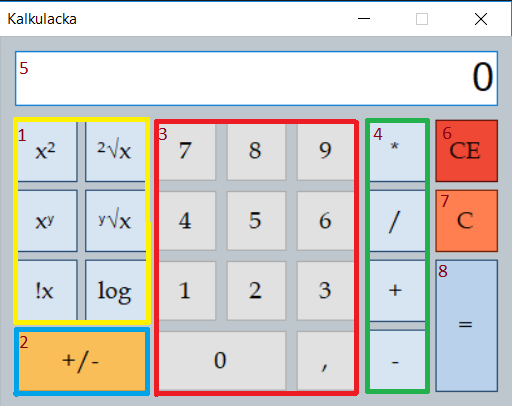
\includegraphics[width=0.6\linewidth]{pictures/1}
		\caption{Výpis čísla} 
	\end{figure}
	
	\textbf{Popis barevných bloků:}
	\begin{enumerate}
	\item Různé operace 
	\item Mění známenko čísla na displeji
	\item Cifry pro práce
	\item Jednoduché operace
	\item Displej
	\item Nastaví displej na 0
	\item Smaže poslední vyraz
	\item Stisknutím dostaneme vysledek
	\end{enumerate}
	\textbf{Poznamky k obr.10 :}
	\begin{enumerate}
	\item Pro počítaní mocniny poprve vybereme číslo (základ), stiskneme tlačitko odmocniny  $x^{y}$ a pak napišeme exponent mocniny
	\item Pro počítaní odmocniny, poprve vybereme číslo (základ), stiskneme	tlačitko odmocniny $\sqrt[y]{x}$ a pak napišeme stupeň odmocniny a "="
	\item Pro počitaní faknorialu, poprve vybereme číslo, pak stiskneme tlačitko faktorial !x
	\end{enumerate}

	\newpage
	
	
	
	
	
	%\begin{figure}[H] 
		%\center\includegraphics[width=0.6\linewidth]{pictures/1_1} 
	%\end{figure}
	
	\newpage
%%%%%%%%%%%%%%%%%%%%%%%%%%%%%%%%%%%%% Závěr %%%%%%%%%%%%%%%%%%%%%%%%%%%%%%%%%%%%%%%%%%%%%%%%%%%%%%%%%%%
	\section*{\LARGE Závěr}
	
	Dekuji za použití produktu od Baseballka. Vaše přaní nebo stížnosti můžete nechat \href{https://github.com/natal1H/IVS-Baseballka} {tady}, v oddílu "Issues"

	
\end{document}